% 
% Annual Cognitive Science Conference
% Sample LaTeX Paper -- Proceedings Format
% 

% Original : Ashwin Ram (ashwin@cc.gatech.edu)       04/01/1994
% Modified : Johanna Moore (jmoore@cs.pitt.edu)      03/17/1995
% Modified : David Noelle (noelle@ucsd.edu)          03/15/1996
% Modified : Pat Langley (langley@cs.stanford.edu)   01/26/1997
% Latex2e corrections by Ramin Charles Nakisa        01/28/1997 
% Modified : Tina Eliassi-Rad (eliassi@cs.wisc.edu)  01/31/1998
% Modified : Trisha Yannuzzi (trisha@ircs.upenn.edu) 12/28/1999 (in process)
% Modified : Mary Ellen Foster (M.E.Foster@ed.ac.uk) 12/11/2000
% Modified : Ken Forbus                              01/23/2004
% Modified : Eli M. Silk (esilk@pitt.edu)            05/24/2005
% Modified : Niels Taatgen (taatgen@cmu.edu)         10/24/2006
% Modified : David Noelle (dnoelle@ucmerced.edu)     11/19/2014

%% Change "letterpaper" in the following line to "a4paper" if you must.

\documentclass[10pt,letterpaper]{article}

\usepackage{cogsci}
\usepackage{pslatex}
\usepackage{apacite}

\usepackage[pdftex]{graphicx} %MJ - Added for graphics
\usepackage{booktabs} % MJ - Added for tables
\usepackage{amsmath} % MJ - Added for equations
\usepackage{verbatim} % MJ - Added for comments
\usepackage{dblfloatfix} % MJ - Added to enable figures at the bottom of page

\title{n-task Learning: Solving Multiple or Unknown Numbers of Reinforcement Learning Problems}
 
\author{{\large \bf Mike Jovanovich and Joshua L. Phillips} \\ 
  (mpj2n@mtmail.mtsu.edu), (Joshua.Phillips@mtsu.edu) \\
  Department of Computer Science \\
  Middle Tennessee State University \\
  Murfreesboro, TN 37132 USA}

\begin{document}

\maketitle

\begin{abstract}
Temporal difference learning models can perform poorly when optimal policy cannot be determined solely by sensory input. Converging evidence from studies of working memory suggest that humans form abstract mental representations that align with significant features of a task, allowing such conditions to be overcome. We here present n-task learning, an algorithm that utilizes abstract representations to form multiple policies based around a common set of sensory inputs. Inputs to a temporal difference learning algorithm are combined conjunctively with an abstract input that comes to represent attention to a task. The agent completes a dynamic categorization problem that is marked by frequently recurring tasks. The algorithm learns the correct number of tasks as well as when to switch from one task representation to another, even when the input is identical across all tasks. Task performance is shown to be optimal only when an appropriate number of abstract representations is used.

\textbf{Keywords:} 
reinforcement learning; temporal-difference learning; task switching; input abstraction

\end{abstract}

\section{\underline{Introduction}}

Functionality typically associated with human and animal working memory has been emulated successfully in computational models that make use of temporal difference (TD) learning algorithms \cite{oreilly_prefrontal_2002,oreilly_making_2006,oreilly_biologically_2006,frank_interactions_2001,kriete_generalisation_2011,kriete_indirection_2013,niv_reinforcement_2015,rougier_prefrontal_2005,phillips_biologically_2005,phillips_working_2006}. While these algorithms can perform well in both stationary and changing environments, their success is contingent upon the ability of the state signal to contain all relevant information for assessing the value of future states (the Markov property) \cite{sutton_reinforcement_1998}. Frequent changes to the optimal policy that are driven by hidden information can confound learning in TD models \cite{sutton_between_1999}.

In this paper we describe n-task learning (nTL), a biologically inspired algorithm that serves as an extension to any member of the TD family of learning algorithms. nTL allows the base algorithm to better handle scenarios in which the agent is required to switch between several tasks with different optimal policies. We show how the model uses abstract task representations (ATRs) to identify and separate the tasks, increasing the efficacy of the base TD learning model. We also demonstrate how the algorithm is able to learn the number of tasks using only the feedback from the critic.

\section{\underline{Background}}

\subsection{Biological Analogs for the Model}

We draw much of the inspiration for our model from work that explores the trade-offs and affordances of both activation and weight based memories. Having multiple mechanisms for storage affords great flexibility in meeting memory demands, and we believe that many of the current computational learning models could benefit from these dual roles.

The nTL algorithm utilizes ATRs to inform policies. These ATRs can be thought of as a kind of filter through which the agent currently perceives the environment. Throughout this section we provide evidence for a biological analog to these ATRs, along with other details relevant to the model, specifically top-down support and dynamic gating in working memory.

O'Reilly et al. (2002) give support for the argument that working memory is responsible for flexibly updating goals. The authors argue that perceptual processing and action selection are influenced by representations that are held in working memory, providing what they describe as ``top-down support'' or ``biasing''. The inability to rapidly switch actively maintained representations results in perseveration on previous learning, as learning must then be accomplished through slower weight based updates. In the same study the authors attempt to show that actively maintained representations in the prefrontal cortex (PFC) are organized by level of abstraction. They cite as evidence behavior exhibited by human patients with frontal damage and experiments performed on monkeys with lesions in this region in the brain.

A later work by Rougier et al. expands on this idea by attempting to provide a model based on PFC-midbrain interaction that develops ``abstract rule-like PFC representations'' \cite{rougier_prefrontal_2005}. This model was trained on multiple tasks where stimuli comprised of features from several dimensions were presented, and reward for each task was determined by a single dimension. The model was contrasted with others lacking various anatomical structures and mechanisms. The authors showed that units in the ``full PFC'' network came to represent all of the features that made up a particular dimension, while other networks tended to form a representation for each stimulus.

We have previously discussed the benefits of being able to actively maintain memories; just as critical is the ability to update concepts that are currently held in memory. It is theorized that this is accomplished in the brain via a system in which the PFC exhibits active maintenance of memory representations and the basal ganglia act as a gate, allowing representations in the PFC to be updated \cite{frank_interactions_2001,chatham_multiple_2015,chatham_corticostriatal_2014,rougier_prefrontal_2005,kriete_indirection_2013,kriete_generalisation_2011}. It has been shown that working memory is updated when levels of the neurotransmitter dopamine are phasically elevated \cite{frank_interactions_2001,chatham_multiple_2015,kriete_generalisation_2011,rougier_prefrontal_2005,niv_reinforcement_2015}. When a reward is expected but not delivered, the resulting negative error signal prompts an update to working memory contents. In addition to flushing retained memory representations and allowing working memory to store new external stimuli, learning is believed to be limited in the presence of a large negative error signal \cite{chatham_multiple_2015,oreilly_biologically_2006}, as can be modeled by the gain parameter to a sigmoidal neural activation function \cite{frank_interactions_2001,oreilly_making_2006}.

\subsection{Relation to Machine Learning Models}

Although the model in this work has some aspects in common with models from other machine learning domains, nTL has a unique property that sets apart from these - the ability to self-monitor and react appropriately based only on reward feedback. The problem that nTL intends to address is one in which contextual cues offer no information that can be used to determine an appropriate action selection policy, such as the Wisconsin Card Sorting Test (WCST). While we see this type of experiment used frequently in psychological literature, we have seen no machine learning models that attempt to solve this problem. In this section we contrast our algorithm with related machine learning works.

Hierarchical reinforcement learning (HRL) bares some similarity to nTL. As an example we use Sutton et al. (1999), in which ``options'' are used as a form of temporal abstraction \cite{sutton_between_1999}. In this case an option is selected and influences action choices until a goal state is reached or the option expires after a predefined number of time steps. An ATR is also an outer abstraction that affects the policy over actions. However, in nTL there is no explicit definition of this abstraction within the algorithm; ATRs are swapped into and out of memory based on task performance rather than predefined conditions. The ability to learn multiple tasks without the use of defined goals is the main contribution of this work. Option-based HRL models are typically used to improve performance on temporally extended tasks with sparse rewards by dividing them into sub-tasks, but are not suited for scenarios in which state representations offer no cues for choosing among options, i.e. when the function for selecting an option is independent of state input. nTL, in contrast, is appropriate when multiple episodic tasks are present, and nothing in the environment is indicative of the task type or duration.

Long short-term memory \cite{hochreiter_long_1997}, or LSTM, has demonstrated success in capturing long-term dependencies and has recently grown in popularity across domains. It is for these reasons that we have chosen it as a state-of-the-art competitor for nTL. Because the response that satisfies the categorization rule is never revealed in the WCST, we have trained the LSTM model with an altered version that minimizes error against the correct response at each trial rather than learning with a reward signal. Although this is not true to WCST form, it allows for comparison against supervised learning algorithms.

\section{\underline{Methods}}

\subsection{Experimental Protocol}
\label{sec:exp}

\begin{figure}[t!]
    \centering
    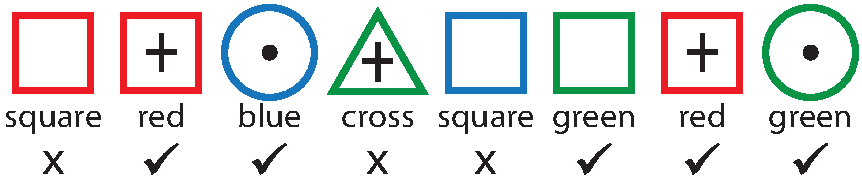
\includegraphics[scale=.55]{images/exp_demo.pdf}
    \caption[]{Shown here is an example round of the experiment with $l$ set to three. Stimuli are composed of three features drawn from three dimensions: color, shape, and fill. The round consists of eight trials. The stimuli are shown in the top row, and the selected action is shown in the middle row. The bottom row designates a correct trial with a check mark, and an incorrect trial with an ``x''. The rule for this round was set to ``color''.}
    \label{fig:exp_demo}
\end{figure}

Our experiment is similar to the dimension selection task described in \cite{rougier_prefrontal_2005}. The agent is presented with a stimulus consisting of $f$ features, selected at random from $d$ dimensions, and is prompted to select one of the features. Feedback is given after each action selection based on whether or not the selected feature matches a categorization rule. The rule corresponds to one of the five dimensions from which the features are drawn, and no cues are given to indicate what this rule is. Correct answers are rewarded by a constant amount, $r_g = 1$. Incorrect answers incur no penalty, $r_d = 0$ . After a predetermined number of consecutive correct responses, $l$, the round is considered learned, and the rule changes (in the style of a WCST). The rule is selected at random, and always differs between two consecutive rounds. Figure \ref{fig:exp_demo} shows an example round.

It is important to note that the distinguishing feature of this problem is that it is composed of several tasks which each must be learned without the use of environmental cues and then remembered while completing the other tasks for success. If something in the environment is present to help the agent determine which rule is currently in effect then the problem becomes a contextual bandit problem. If the tasks are not repeated then the problem becomes a non-stationary bandit problem. Without a way to associate learning with a task representation the agent effectively treats the WCST as a non-stationary bandit problem, and performance suffers due to perseveration after rule changes (as is later shown). 

The decision to directly align categorization rules with the dimensions of the stimuli was made in order to more easily draw conclusions from existing cognitive science research. Categorization rules represent the set of action choices that lead to reward, and may be chosen arbitrarily.

\subsection{Key Terms}

\begin{itemize}
\item In a particular experiment some dimensions may never be used for the categorization rule, and serve only as distractors. We refer to the number of distinct rules that are used throughout the experiment as the number of \textit{tasks}. 
\item A \textit{trial} consists of one presentation of a stimulus to the agent, the choosing of an action by the agent, and a reward value given to the agent by the critic. This is equivalent to a single time step in the reinforcement learning framework. 
\item A \textit{round} consists of all of the trials completed by the subject during one completion of a task, from the time a new categorization rule is put into effect to the time the subject has completed $l$ consecutive correct trials. 
\item When the model substitutes an ATR that is in memory with one that is not in memory we call this a \textit{task switch}. 
\end{itemize}

\subsection{Holographic Reduced Representations}
\label{sec:hrr}

Unitary holographic reduced representations (HRRs) \cite{plate_holographic_1995} are used in our experiments to encode state and action inputs. With HRRs, features are distributed over the width of an entire vector of $ n $ elements rather than tied to a particular position or index in a vector. Conjunction and disjunction of input features is accomplished mathematically by circular convolution and addition of vectors respectively. As a result, relationships between concepts are represented without increase in dimensionality. 

Although we use an HRR framework for encoding in this work we do not believe the results obtained are contingent upon this choice, and we see no reason why alternate encodings such as vectors \cite{mitchell_composition_2010}, tensors \cite{papalexakis_tensors_2016}, or spatio-temporal encodings \cite{hummel_distributed_1997} could not produce similar results.

\subsection{Working Memory Computational Model}

In order to see the consequences of the ATR mechanism, we will first describe the working memory model as it functioned prior to the addition of ATRs, which are described in the following subsection. The state (the feature set that comprises the current trial) is in the form of a single HRR, which is the result of disjunctively combining the components of the stimuli. In our experiments the action choices correspond directly to the features in the environment. To differentiate between a particular feature in the state role (e.g. ``seeing red'') and the same feature in the action role (``selecting red''), these corresponding states / actions are comprised of different HRRs.

At each trial the model updates the predicted value of choosing a particular action for a particular state through use of the SARSA algorithm. The $ Q $ function for SARSA is approximated using a single-layer perceptron neural network with a linear activation function. Because of this architecture, the output for the network is simply the dot product of the input HRR and a weight vector plus a scalar bias term, $b$, as shown in Equation \ref{eq:action_selection}. This weight vector is initialized in the same way as HRRs, and the bias term is set to the reward level that will be received upon reaching the goal state. Setting the bias in this way has the effect of encouraging exploration via optimistic initial values (``optimistic critic''). To counter the eventual decrease in exploration that comes from overcoming the initial optimism we also implement an $ \epsilon $-soft policy that makes non-greedy decisions a small fraction ($\epsilon$) of the time.  

An action is selected by forming the conjunct representation of state with each candidate action for the trial, and using the resultant representations as inputs into the $ Q $ function. The action that yields the greatest value, $m$, is then chosen. This can be formulated as:

\begin{equation}
m = \underset{c \in C}{argmax}((s \wedge c) \cdot w_{q}+b)
\label{eq:action_selection}
\end{equation}

\noindent where $ s $ is the current state representation, $ C $ is the set of all candidate action choices for the current trial, and $ w_{q} $ is the weight vector for the $ Q $ function neural network. At each trial the reward is used to update weights for the $Q$ function. In order to make learning more stable a log-modulus transformation \cite{john_alternative_1980} is applied to the error during updates to the $ Q $ function, $ A $ function (introduced in the next section), and $t$ threshold (introduced in next section). This transformation mitigates learning instability due to relatively large errors (data not shown):

\begin{equation}
\Delta w_i = \alpha_q [sgn(\delta) * log(| \delta | + 1) * (s \wedge m)_i]
\label{eq:weight_update_transform}
\end{equation}

In the above equation, $ w_i $ indicates the value of the weight vector at index $ i $, $ \alpha_q $ is the learning rate, $ \delta $ is the error, and $ (s \wedge m)_i $ is the value of the HRR input vector (the eligibility trace) at index $ i $. Although we are using SARSA to learn a policy for action selection, the experiment does not model a temporally extended task. Since all feedback is relevant to only a single trial, we have set the $\lambda$ and $\gamma$ TD parameters to zero, and all updates are treated as goal state updates.

\subsection{n-task Learning Algorithm}
\label{sec:n-task}

\begin{figure}[t!]
    \centering
    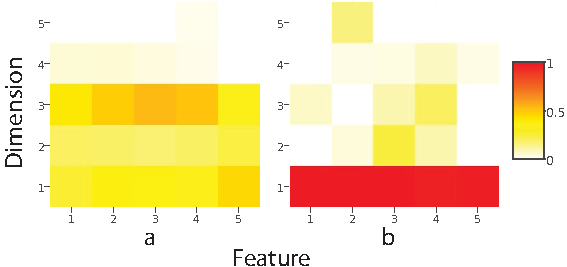
\includegraphics[scale=.65]{images/actionvals_hm.pdf}
    \caption[]{Shown here are feature selection values for all features in the state set. \textit{a} shows results from a trial taken near the beginning of a round after 100 rounds of training using traditional SARSA (the single ATR case) to learn three tasks. Although the categorization rule for this trial is dimension one, we see that action values along dimension three, the rule from the previous round, are highest. By contrast, when three ATRs are used, as in \textit{b}, we see the formation of clear dimensional representations after 100 rounds of training.}
    \label{fig:actionvals_hm}
\end{figure}

\begin{figure*}[t!]
    \centering
    \begin{minipage}{0.48\textwidth}
        \centering
        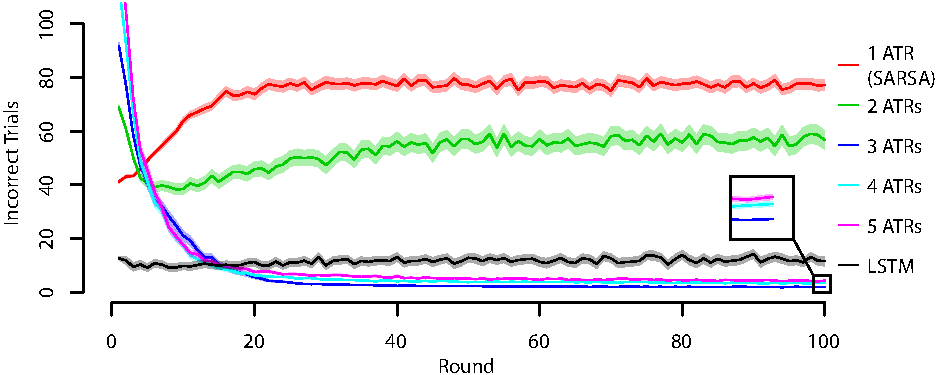
\includegraphics[scale=.53]{images/task_performance.pdf}
        \caption[]{Static nTL - shown here are the average number of incorrect trials taken at each round. mean values for 1000 runs are shown by the solid lines, with shading to show a 95\% confidence interval. the number of tasks, $n$, is three. performance will converge to a theoretically optimal $ n/2 $ incorrect trials per round on average when $ n $ atrs are used.}
        \label{fig:task_performance}
    \end{minipage}\hfill
    \begin{minipage}{0.48\textwidth}
        \centering
          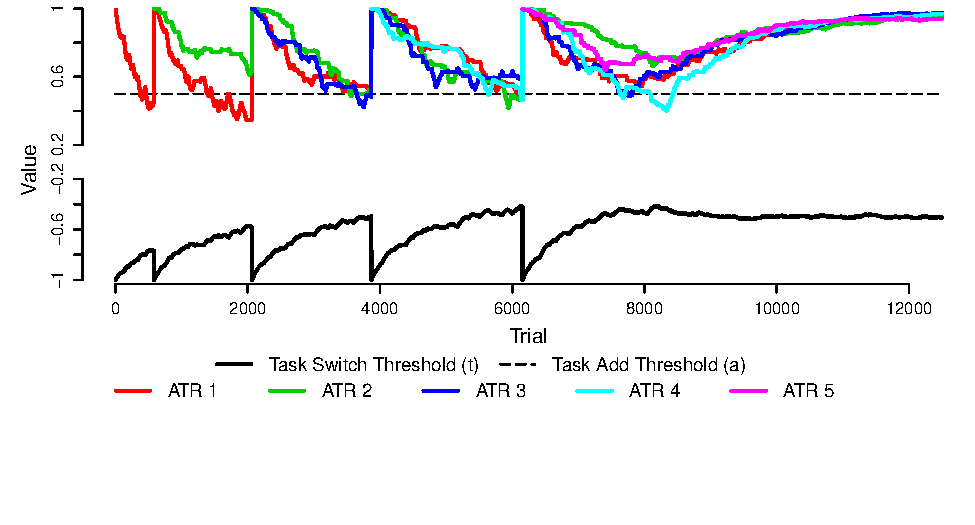
\includegraphics[scale=.53]{images/learn_num_tasks.pdf}
          \caption[]{Dynamic nTL - ATR values for a scenario in which the number of task representations adapts to achieve optimal performance. The number of categorization rules in this experiment was five.}
          \label{fig:learn_num_tasks}
    \end{minipage}\hfill
\end{figure*}
        
As mentioned earlier, nTL can be viewed as an extension to a standard TD learning algorithm, which we call the base algorithm. We have used SARSA as the base algorithm for our experiments, but other TD learning algorithms could be substituted. At the heart of this approach is the idea that any input can be bound to a task by forming the conjunct of the original input and another input that uniquely identifies an ATR. The ATR inputs are created arbitrarily, and encoded in the same way as the input features. The algorithm requires a function, $A$, to keep keep track of the value of each ATR. For this we simply maintain and update a vector of values that are mapped to the ATRs. If desired, a neural network could also be used to model the ATR values.
   
Before any input is fed into the base algorithm the input is conjunctively joined with the ATR representation that is currently in memory, $atr$. In this way a single input can take on multiple values by being bound to different ATRs and presented to the base algorithm. No alterations to the base algorithm are required in order for this approach to work. Our action selection equation now becomes:

\begin{equation}
m = \underset{c \in C}{argmax}((s \wedge c \wedge atr) \cdot w_{q}+b)
\label{eq:action_selection_atr}
\end{equation}

\noindent The weight update is modified in a similar manner; where before in Equation \ref{eq:weight_update_transform} we had only $s \wedge m$ to represent the input to SARSA, now we must include the selected ATR. The new input is $s \wedge m \wedge atr$. In short, $Q(s,m)$ becomes $Q(s,m,atr)$.

Reward feedback from each trial is used to update the value of the current ATR. The error used for this update is simply the TD error for the ATR value function. In the below equation, $A$ is the function determining the ATR values, $ \alpha_a $ is the learning rate for ATRs, and $\delta$ is $r - A(atr)$. Note that in our experiments, the $A$ function also uses optimistic initial values, so all ATRs start with a value equal to the goal state reward:

\begin{equation}
A(atr) \leftarrow A(atr) + \alpha_a [sgn(\delta) * log(|\delta| + 1)]
\label{eq:a_function_update}
\end{equation}

Trials that result in a task switch do not incur an update to the $A$ or $Q$ functions. In this way the current ATR is not penalized for a task change that is external to the agent. Although we do not give data here, this adaptation leads to $ A $ values that are more stable (show less fluctuation) and that converge to the average reward values for trials within the tasks.

The model determines when to switch to a new ATR via a threshold, $ t $. When the TD error ($\delta=r-Q(s,m,atr)$) is less then $ t $, this signals to the model that the current ATR is not well suited to handle current input, and the next sequential ATR is subbed in for the current one. This $t$ value is first initialized to negative one times the reward for the goal state, and is updated at each trial using the TD error from the $Q$ function, where $ \alpha_t $ is the learning rate for $t$:

\begin{equation}
t \leftarrow t - \alpha_t [sgn(\delta) * log(|\delta| + 1)]
\label{eq:t_update}
\end{equation}

In the case that the number of tasks is known ahead of time, the number of ATRs can be set explicitly. We refer to this as static nTL. In many cases the number of tasks is unknown, or changes with time. In dynamic nTL the number of ATRs is set automatically based on task performance. To accomplish this an additional task add threshold, $a$, is needed to determine the number of ATRs to maintain. Whenever a task switch occurs $ A $ values for all ATRs are averaged. If this mean value falls below $ a $ then a new ATR is added, and both $ A $ and $ t $ are reinitialized. Unlike $ t $, the $ a $ threshold is constant. Although any biological analog for this threshold would likely be dynamic, we have not yet found a way to model this behavior.

The model starts with a single ATR in dynamic nTL, and grows toward the optimal number of representations. This aligns with research showing that humans and animals assume a simple task structure in dynamic categorization tasks in which reward is determined by a single dimension, and move on to more complex hypotheses only after exhausting all simple ones \cite{shepard_learning_1961}.

\subsection{Additional Details for Experiment Setup}

\begin{table}[!b]
{\small
  \caption{Parameter Descriptions and Values }
  \label{tab:parameters}
  \centering
  \begin{tabular}{lll}
    \toprule
    \midrule
    \textbf{Name}     & \textbf{Value}    & \textbf{Description}   \\
    $ l $   & 8         & Consecutive correct trials to complete a round \\
    $ d $   & 5         & Dimensions for task stimuli \\
    $ f $   & 5         & Features in each dimension \\
    $ n $   & 1024      & Size of HRR vectors \\
    $ \epsilon $ & 0.005 & Probability for non-greedy action choice \\
    $ \alpha_q $ & 0.05  & Learning rate for the $ Q $ function update \\
    $ \alpha_a $ & 0.0075 & Learning rate for the $ A $ function update \\
    $ \alpha_t $ & 0.002 & Learning rate for the $ t $ threshold update \\
    \bottomrule
  \end{tabular}
}
\end{table}

A list of parameter values is provided in Table \ref{tab:parameters}. Parameters for all models were chosen by minimizing the mean number of incorrect trials over 100 tasks for 100 random runs of the experiment. All listed nTL results were obtained using R version 3.4.0. The source code used for these experiments can be downloaded freely from: \url{https://github.com/mpjovanovich/ntask\_learning}

The LSTM model was built using TensorFlow version 1.3.1. This model performed best with a learning rate of 7.0, and a state size of one. Results remained the same for all state sizes in the tuning range. The model was trained after each trial using the most recent ten trials. Tuning ranges were as follows, with a step size of 0.05: learning rate (0,10], state size [1,20], trials used for training [1,40].

\section{\underline{Results}}

Two experiments were conducted using the previously described protocol. In the first experiment the appropriate number of ATRs is known \textit{a priori}, so we use static nTL. In the second, the number of ATRs is learned using dynamic nTL. 

\subsection{Experiment 1 - Static n-task Learning}

Figure \ref{fig:task_performance} shows how task performance changes as a function of the number of ATRs being used. Three tasks were present in this experiment. Although a statistically significant difference is shown between all results, we see that having too few ATRs is much more detrimental to performance than having too many. When compared to the case when the number of ATRs was equal to the number of tasks (3 ATRs), having one too few (2) ATRs resulted in 2782\% more incorrect trials per round after 100 rounds, whereas having one too many (4) ATRs resulted in only 81\% more incorrect trials per round. The LSTM model resulted in a 487\% increase in incorrect trials, and traditional SARSA gave a 3827\% increase.

By setting the number of ATRs to one, we simulate the behavior of an agent that is not capable of learning dimensional representations. This is equivalent to standard TD learning, in this case SARSA. We would expect such an agent to perseverate on previously learned features when a task switch occurs, and the results confirm that perseveration occurs. When only one ATR is available, many incorrect trials are taken in each round (see Figure \ref{fig:task_performance}). When a rule change occurs, action choices that were valuable in the previous round are tried first (see Figure \ref{fig:actionvals_hm}a). Only after a period of unlearning the previous external task does the model begin to select new actions. 

We see from Figure \ref{fig:actionvals_hm}b that when the number of ATRs is equal to the number of external tasks, each ATR comes to represent the dimension for one external task. This is because after the initial learning and exploration period each ATR is used only for the subset of trials that correspond to an external task. If an ATR is used on a trial that results in a task switch, no weight updates take place.

\subsection{Experiment 2 - Dynamic n-task Learning}

Here we illustrate dynamic nTL with a five task example (see Figure \ref{fig:learn_num_tasks}). Trials where $t$ drops to the starting value indicate that the mean ATR value exceeded $a$, and an ATR was added. When five ATRs were present, the mean ATR value remained above $a$ during initial exploration, and eventually converged to the value of the goal state reward. Because the first experiment provided the data needed to compare against models lacking a mechanism for the formation of ATRs, no additional models were used for comparison in this experiment.

\section{\underline{Discussion}}

Discussing the nTL model in terms of a human actor allows us to more easily connect to previously discussed biological models. When the agent expects to receive a reward and none is given, the resulting negative error signal cues the agent to try a new strategy (switch to a new ATR), and no learning takes place. There is initially a period of rapid task switching as the agent gives many incorrect responses due to exploration and lack of learning. After a time the estimated feature selection values that are associated with each ATR stabilize, and internal task switching (swapping a new ATR into memory) occurs only in response to a true external task switch.

The ATRs influence the agent's thinking about the current trial through a mechanism of top-down support \cite{oreilly_prefrontal_2002}. If we take a single trial representation and associate it with two different ATRs, the agent will have a different assessment of value for each. Let us suppose that the agent is presented with a small red circle as stimulus, and the action candidate ``select red''. When the first ATR is present in memory this action may have a high value, but when the second ATR is in memory the value is low. We can then conclude that the first ATR has come to represent a task in which selecting red when seeing these stimuli leads to reward, and the second to represent a task in which seeing red does not lead to reward (this second ATR may have been used for a shape or size categorization task). In this way the switching of ATRs effectively becomes a filter for possible actions. The agent attends to a different subset of actions with each successive trial, iterating through hypotheses that have lead to prior success as it attempts to find one that fits the task.

We have shown that an agent with only a single ATR will perseverate when a rule change switch occurs. In this case there is a period during which the previously learned task is unlearned, followed by a period in which the new task is learned. This scenario simulates learning without activation based memories, where all learning must be accomplished through weight updates \cite{oreilly_prefrontal_2002}.

When the number of ATRs matches the number of tasks, the mean of the agent's estimated values for the ATRs (the $ A $ function) converges to the goal reward value of the tasks. When too few ATRs are present this mean declines to a value that is below the goal reward. Using these two observations, we can set a threshold ($a$) that acts as a cutoff point for overall ATR performance. When the mean value falls below this threshold the agent increases the complexity of its thinking by adding another ATR, until the number of ATRs is equal to the number of tasks.

One notable deviation from human-like thinking in the dynamic nTL model is that previous learning is discarded when an ATR is added. The reason for ``resetting'' when we reach this point is to keep the task switch threshold, $t$, in a range that will cause ATRs to be switched appropriately. If previous $Q$ learning is retained (by leaving intact the $Q$ neural network) and $t$ is reset, then $t$ will remain too low, resulting in too few task switches for ATRs to effectively represent the tasks. If previous $Q$ learning is retained and $t$ is not reset, then $t$ will climb too high, resulting in a task switch for every trial. It is for this reason that we both reinitialize the $Q$ weight vector and reset the task switch threshold when tasks are added.

While we believe nTL can be used to great benefit for dynamic tasks such as the one used in this experiment, we recognize that it is not appropriate for all reinforcement learning scenarios. Specifically, we have only tested the algorithm in the case where reward is constant and able to be achieved at each time step, the task distribution is uniformly stochastic, the number of tasks does not change, and all features are used for a single categorization rule at most. A model that is able to accommodate variable/probabilistic rewards, temporally extended tasks, adversarial task distributions, and the introduction and removal of tasks could be extremely useful. We would be interested to see more research on the means by which humans come to learn the number of tasks present in a given scenario, both to provide biological inspiration for further work and to assess plausibility of the current model.

\setlength{\bibleftmargin}{.125in}
\setlength{\bibindent}{-\bibleftmargin}

\bibliographystyle{apacite}
\bibliography{references}

\end{document}
